\documentclass{article}
\usepackage{fancyhdr,amssymb,amsmath,amsthm,bbm,enumerate,mdwlist,url,multirow,hyperref,graphicx,dsfont}
\usepackage{pdfpages}
\usepackage{algorithm}
\usepackage{algpseudocode}
\addtolength{\hoffset}{-1.5cm}
\addtolength{\textwidth}{3cm}
\addtolength{\voffset}{-1.5cm}
\addtolength{\textheight}{3cm}


\usepackage[slovene]{babel}
 \usepackage[utf8]{inputenc}
\usepackage[T1]{fontenc}
\usepackage{graphicx}


\begin{document}
\newtheorem{definition}{Definicija}


\title{Graphs of type (SB) and domination on their cartesian products}

\author{Jan Hrastnik, Matic Kremžar}
\date{11. 12. 2024}
\maketitle


\section{Uvod}
V projektni nalogi sva se ukvarjala z grafi tipa (SB) in dominacijo na njihovem kartezičnem produktu. 
Projektna naloga je bila izvedena v programu SageMath, obsežni izračuni pa s pomočjo spletne strani CoCalc.
Naloga ima odprt tudi svoj repozitorij na GitHubu, na naslovu https://github.com/matickremzar/Graphs-of-type-SB-and-domination-on-their-cartesian-products-/tree/main.
Tam so zbrane tudi vse datoteke, ki sva jih uporabila med izdelavo projekta.

Cilj je razumeti, kako prepoznati, konstruirati in spreminjati grafe tipa (SB), 
ter analizirati njihove lastnosti, zlasti dominacijsko število njihovih kartezičnih produktov.

\section{Osnovna ideja in definicije}
Delala sva z usmerjenimi grafi $G = (V,E)$, kjer je $G$ množica vozlišč, $E$ 
pa množica povezav grafa.

\begin{definition}
    Graf $G$ je tipa $(SB)$, če je njegov premer enak $2$ in ima dve sosednji vozlišči $v_1, v_2\in V$, da velja:
    \begin{itemize}
        \item $v_1$ in $v_2$ nimata skupnega soseda,
        \item $G$ ima vozlišče $v^*\in V$, ki ni sosednje $v_1$ ali $v_2$; torej $v^*\not\sim v_1$ in $v^*\not\sim v_2$. \newline
    \end{itemize}
\end{definition} 

\begin{figure}[h!]
    \centering
    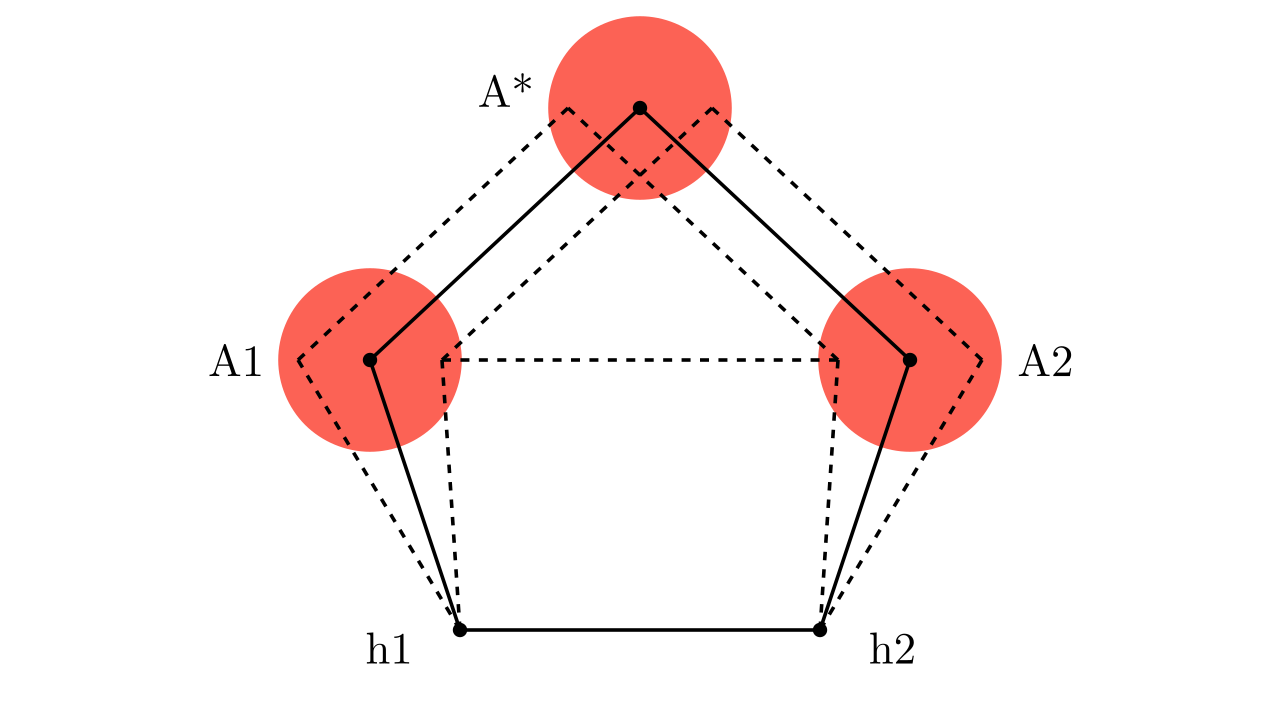
\includegraphics[width=0.5\textwidth]{GraphPlanarDegrees_ManimCE_v0.18.1.png} % 0.5 pomeni pol širine strani
    \caption{Skica grafov tipa (SB)}
    
\end{figure}

Zapišemo lahko particijo vozlišč grafa $G$ kot $$V(G) = {v_1, v_2} \cup A_1 \cup A_2 \cup A^*,$$
kjer je $A_1$ množica vozlišč, ki so sosednja $v_1$, $A_2$ množica vozlišč, ki so sosednja $v_2$ in 
$A^*$ množica vozlišč, ki niso sosednja niti $v_1$ niti $v_2$.

\begin{definition}
   Podmnožica vozlišč $D\subseteq V$ grafa $G=(V,E)$ se imenuje \emph{dominacijska množica} grafa,
   če je vsako vozlišče $v\in V$ grafa v množici $D$, ali pa je kakšno njemu sosednje vozlišče
   v $D$. \emph{Dominacijsko število $\gamma(G)$} grafa je velikost najmanjše dominacijske
   množice grafa.
\end{definition}

\begin{definition}
    Kartezični produkt $G\square H$ grafov $G$ in $H$ je graf, za katerega velja:
    \begin{itemize}
        \item vozlišča grafa $G\square H$ so kartezični produkt $V(G)\times V(H)$,
        \item dve vozlišči $(u,v)$ in $(u',v')$ sta sosednji v grafu $G\square H$ natanko tedaj, ko je:
        \begin{itemize}
            \item $u=u'$ in $v$ je sosed $v'$ v $H$, \textbf{ali}
            \item $v=v'$ in $u$ je sosed $u'$ v $G$.
        \end{itemize}
    \end{itemize}
\end{definition}

\section{Naloga 1}
\subsection{Preverjanje, ali je graf tipa (SB)}
Sprva je potrebno zapisati kodo, ki preveri, ali je dan graf tipa (SB) (v datoteki $sb\_detect\_koncna.py$). Uporabimo matriko sosednosti. Dovolj je, 
da pregledamo zgolj zgornji trikotnik matrike, saj tako že pridobimo vse podatke o sosedih. Nato 
preverimo še veljavnost prej zapisanih lastnosti grafov tipa (SB).



\begin{algorithm}
\caption{Preverjanje, ali je graf tipa (SB)}
\begin{algorithmic}[1]
\Function{IsSB}{G: Graph} \Comment{Funkcija za preverjanje grafa tipa (SB)}
    \State \textbf{if} $G.diameter() \neq 2$ \textbf{then} \Return \textbf{False} \Comment{Premer mora biti 2}
    \State $adj \gets G.adjacency\_matrix()$ \Comment{Pridobimo matriko sosednosti}

    \For{$i \gets 1$ \textbf{to} $adj.nrows()$}
        \For{$j \gets i+1$ \textbf{to} $adj.nrows()$} \Comment{Samo zgornji trikotnik}
            \If{$adj[i, j] = 1$} \Comment{Če sta $i$ in $j$ soseda}
                \State $common\_neighbour \gets \textbf{False}$
                \For{$k \gets 1$ \textbf{to} $adj.nrows()$}
                    \If{$adj[i, k] = 1$ \textbf{and} $adj[j, k] = 1$} \Comment{Preverimo skupne sosede}
                        \State $common\_neighbour \gets \textbf{True}$
                        \State \textbf{break}
                    \EndIf
                \EndFor
                \If{$common\_neighbour$}
                    \State \textbf{continue}
                \EndIf

                \State $nonadj\_vertex\_exists \gets \textbf{False}$
                \For{$k \gets 1$ \textbf{to} $adj.nrows()$}
                    \If{$adj[i, k] = 0$ \textbf{and} $adj[j, k] = 0$ \textbf{and} $k \neq i$ \textbf{and} $k \neq j$}
                        \State $nonadj\_vertex\_exists \gets \textbf{True}$
                        \State \textbf{break}
                    \EndIf
                \EndFor

                \If{$nonadj\_vertex\_exists$}
                    \State \Return \textbf{True}
                \EndIf
            \EndIf
        \EndFor
    \EndFor

    \State \Return \textbf{False} \Comment{Graf ni tipa (SB)}
\EndFunction
\end{algorithmic}
\end{algorithm}


\subsection{Iskanje vseh grafov tipa (SB) na do 10 vozliščih}

Najprej sva v datoteko $diam\_two\_graphs.txt$ zbrala vse grafe s premerom 2 na do 10 vozliščih.
Nato sva te grafe prefiltrirala s spodnjo kodo in podatke zbrala v novi datoteki 
$sb\_graphs.txt$, ki je dostopna preko hiperpovezave v README datoteki na GitHub repozitoriju projekta.
Datoteka je velika privližno 400 MB.

\begin{algorithm}
    \caption{Filtriranje grafov tipa (SB)}
    \begin{algorithmic}[1]
    \State Odpri datoteko \texttt{'sb\_graphs.txt'} v načinu dodajanja (\texttt{"a"}).
    \State Odpri datoteko \texttt{"diam\_two\_graphs.txt"} v načinu branja (\texttt{"r"}).
    \For{\textbf{vsako} vrstico $line$ v datoteki \texttt{"diam\_two\_graphs.txt"}}
        \State $g \gets \textbf{pretvori\_v\_graf}(line)$ \Comment{Ustvari graf iz podatkov na trenutni vrstici.}
        \If{$is\_sb(g)$} \Comment{Preveri, če je graf $g$ tipa (SB).}
            \State Zapiši $line$ v datoteko \texttt{'sb\_graphs.txt'}.
        \EndIf
    \EndFor
    \State Zapri obe datoteki.
    \end{algorithmic}
\end{algorithm}

Z zadnjo kodo še preverimo, koliko je grafov tipa (SB) za posamezen $n$ (število vozlišč), manjši ali enak 10.
Rezultati so prikazani spodaj.



\begin{algorithm}
    \caption{Preštevanje grafov tipa (SB) z različnim številom vozlišč}
    \begin{algorithmic}[1]
    \State counter $\gets$ [0, 0, 0, \dots, 0] \Comment{ (seznam s 11 ničlami, za štetje grafov z različnim številom vozlišč)}
    \State \textbf{Odpri datoteko $'sb\_graphs\_g6.txt'$}
    \For {vsako vrstico $line$ v datoteki}
        \State $g \gets \textbf{pretvori\_v\_graf}(line)$ \Comment{ (ustvarimo graf iz vrstice)}
        \State counter[\text{len}(g.\text{vertices}())] $\gets$ counter[\text{len}(g.\text{vertices}())] + 1
    \EndFor
    \State \textbf{Izpis rezultatov:}
    \For {vsak i od 0 do 10}
        \State izpiši "Število grafov tipa (SB) z $i$ vozlišči: counter[i] "
    \EndFor
    \end{algorithmic}
 \end{algorithm}

 \begin{table}[h!]
    \centering
    \begin{tabular}{|c|c|}
    \hline
    \textbf{n (število vozlišč)} & \textbf{Število grafov tipa (SB)} \\
    \hline
    0 & 0 \\
    1 & 0 \\
    2 & 0 \\
    3 & 0 \\
    4 & 0 \\
    5 & 2 \\
    6 & 11 \\
    7 & 116\\
    8 & 1688\\
    9 & 43420 \\
    10 & 2079097 \\
    \hline
    \end{tabular}
    \caption{Tabela števila grafov tipa (SB) glede na število vozlišč}
    \end{table}

\section{Naloga 2}

Namen te naloge je naključno konstruirati grafe tipa (SB) za večje $n$.
Vzamemo nek graf na $n$ vozliščih in ga s pomočjo smiselnega odvzemanja in dodajanja povezav 
(poskušamo doseči na particijo vozlišč, da pridobimo pogoje za (SB)) poskušamo 
spremeniti v graf tipa (SB). Pri tem moramo paziti na premer.


\begin{algorithm}
    \caption{Generiraj naključen SB graf - naloga 2}
    \begin{algorithmic}[1]
    \State \textbf{Vhod:} Celo število $n$ (število vozlišč)
    \State \textbf{Izhod:} Graf $g$ tipa SB z premerom 2
    \State $g \gets$ Naključen graf z $n$ vozlišči in verjetnostjo povezave 0.5
    \State $(h1, h2) \gets$ prvi rob grafa $g$
    \State $a1 \gets$ sosedi vozlišča $h1$
    \State $a2 \gets$ sosedi vozlišča $h2$
    \State Odstrani $h2$ iz seznama $a1$
    \State Odstrani $h1$ iz seznama $a2$
    \State $a\_star \gets$ prazen seznam
    \For {vsako vozlišče $v$ v grafu $g$}
        \If {$v \notin a1$ in $v \notin a2$ in $v \neq h1$ in $v \neq h2$}
            \State Dodaj $v$ v seznam $a\_star$
        \EndIf
    \EndFor
    \State $vertices\_to\_remove \gets$ prazen seznam
    \For {vsako vozlišče $n1$ v $a1$}
        \For {vsako vozlišče $n2$ v $a2$}
            \If {$n1 == n2$}
                \State Odstrani rob $(h1, n1)$
                \State Dodaj $n1$ v seznam $vertices\_to\_remove$
            \EndIf
        \EndFor
    \EndFor
    \For {vsako vozlišče $v$ v seznamu $vertices\_to\_remove$}
        \State Odstrani $v$ iz seznama $a1$
    \EndFor
    \If {dolžina seznama $a1$ je 0}
        \State $u \gets$ dodaj novo vozlišče
        \State Dodaj $u$ v seznam $a1$
        \State Dodaj rob $(h1, u)$
    \EndIf
    \If {dolžina seznama $a2$ je 0}
        \State $u \gets$ dodaj novo vozlišče
        \State Dodaj $u$ v seznam $a2$
        \State Dodaj rob $(h2, u)$
    \EndIf
    \If {dolžina seznama $a\_star$ je 0}
        \State $u \gets$ dodaj novo vozlišče
        \State Dodaj $u$ v seznam $a\_star$
        \State $v_{a1} \gets$ prvi element seznama $a1$
        \State $v_{a2} \gets$ prvi element seznama $a2$
        \State Dodaj rob $(u, v_{a1})$
        \State Dodaj rob $(u, v_{a2})$
    \EndIf
    \For {vsako vozlišče $u$ v seznamu $a1$}
        \For {vsako vozlišče $v$ v seznamu $a\_star$}
            \State Dodaj rob $(u, v)$
        \EndFor
    \EndFor
    \For {vsako vozlišče $u$ v seznamu $a2$}
        \For {vsako vozlišče $v$ v seznamu $a\_star$}
            \State Dodaj rob $(u, v)$
        \EndFor
    \EndFor
    \State $diam \gets$ premer grafa $g$
    \If {$diam == 2$ in $g$ je tipa SB}
        \State \textbf{Vrni} graf $g$
    \EndIf
    \end{algorithmic}
    \end{algorithm}
    

\section{Naloga 3}

Želimo pridobiti tudi nov graf tipa (SB) iz danega grafa tipa (SB) tako, 
da naredimo nekaj manjših naključnih modifikacij (npr. dodajanje/odvzemanje 
vozlišč/povezav). 
\\
Koda je dostopna v datoteki $random\_modify\_SB\_graph.py$ na GitHubu, zaradi 
dolžine pa je zapisana le glavna ideja programa. 
\\Funkcija $random\_modify\_sb\_graph$ kot argument vzame graf tipa (SB) in 
ga najprej shrani (kot varovalo za kasneje, če naključne spremembe ne dajo 
grafa tipa (SB)). Zapiše particijo vozlišč in se odloči za naključno število 
naključnih sprememb iz nabora. Te spremembe so same po sebi lahke za sprogramirati, paziti 
je treba zgolj, da ne prihaja do kakšnih neželenih struktur (samozanke ...). Število sprememb je na začetku kolikor toliko majhno, da ne tvegamo,
da bi graf preveč spremenili iz tipa (SB). Program izvede te spremembe in preveri ali nov graf ustreza tipu (SB).
V kolikor ne, se postopek na takšnem grafu nadaljuje do tisočkrat, kasneje pa 
spet začnemo z originalnim grafom, ker bi bil novi graf lahko že precej degeneriran.
\\
Funkcijo sva stestirala na približno 5000 primerih, pri čemer je za $n$ blizu $30$ postopek 
v okoli $95 \%$ primerov vrnil graf tipa (SB) preden je bilo izvedenih $1000$ poskusov, torej preden smo  
spet vzeli prvotni graf. Skoraj vedno, ko je bilo generiranje grafa uspešno v teh prvih $1000$ poskusih,
se je to zgodilo v prvih $5$ poskusih, kar potrjuje smiselnost zaustavitvenega pogoja z \emph{while} zanko.
Sklepava, da so namreč bili grafi potem že zelo 'oddaljeni' od tipa (SB). Za velike $n$ je bil pri teh neuspešnih 
poskusih verjetno največkrat problem, da se je povečal premer grafa.

\section{Naloga 4}

Poglejmo za začetek dominacijsko število na običajnih grafih tipa (SB).
Intuitivno jasno je, da imajo vsi grafi tipa (SB) dominacijsko število najmanj 2. Tudi dokaz je jasen:
Zapišimo particijo vozlišč nekega grafa tipa (SB), kot je predlagano v osnovni ideji problema.
Če je v najmanjši dominacijski množici vozlišče $v_1$, imamo zraven pokrito še $v_2$ in 
$A_1$. Vemo pa, da je $A^*$ neprazna, saj obstaja vozlišče $v^*$, ki ni 
sosednje $v_1$ ali $v_2$. Torej $v_1$ ni zadosten in potrebujemo vsaj še eno vozlišče v dominacijski množici.
Analogno sledi za $v_2$. Če je v dominacijski množici neko vozlišče iz $A^*$ ali $A_2$ ($A_1$), rabimo še neko
vozlišče, ki je sosedno $v_1$ ($v_2$). 
\\
V praksi se je izkazalo, da ima velika večina grafov tipa (SB) na do $10$
vozliščih dominacijsko število enako $2$, preostali pa $3$. 
\\
Nato lahko vpeljemo Vizingovo domnevo: Za grafa G in H velja
$$ \gamma(G)*\gamma(H) \leq \gamma(G\square H). $$
Ta sicer ni dokazana v splošnem, je pa preverjena za zadosten nabor grafov, da jo je smiselno uporabiti v 
tej nalogi.
Iz tega lahko trdimo, da je najnižje možno dominacijsko število na 
kartezičnem produktu dveh grafov tipa (SB) enako $4$. 
\\
Zanimiva variacija problema bi bila, v kolikor bi bil kartezični produkt nekih
dveh grafov tipa (SB) spet graf tipa (SB). Posledično bi takoj sledilo, da obstajajo 
grafi tipa (SB) z dominacijskim številom vsaj $4$. Ko sva pregledala grafe na do $10$ vozliščih, 
takšnega primera nisva našla. Problem je bil seveda premer kartezičnih produktov grafov. Vseh $125000$ grafov, ki 
sva jih tako generirala je imelo premer $4$.
\\
Iskanje zgornjih mej za dominacijsko število kartezičnega produkta dveh grafov tipa (SB) je zahtevnejša.
Najboljša zgornja meja, ki sva jo uspela najti je še ena Vizingova izpeljava:
$$ \gamma(G\square H) \leq min\{\gamma(G)\lvert H \rvert, \gamma(H)\lvert G \rvert\}$$



\end{document}
